%In this case, the familiar structure functions  $F_1$, $F_2$, $g_1$, and $g_2$ which describe
%inclusive scattering of electrons from spin-1/2 targets, must be supplemented for a spin-1 system
%by four additional structure functions : $b_1$, $b_2$, $b_3$, and $\Delta$.
%
%
%The tensor structure function $b_1$, ( which is leading-twist like  $F_1$ and $g_1$), is quite
%interesting, in that it presents a simple gauge of nuclear effects: $b_1$ would vanish if the
%deuteron was simply a proton and neutron in a relative S state.
%
%Nuclear effects/EMC effect
%%When spin physics joins naturally the nuclear effects area and model independent
%%nuclear effects extraction compared to polarized EMC effect.
%
%Exotic components.
%
%The Hermes collaboration  made a first measurement~\cite{Airapetian:2005cb} of
%$b_1$ and found significantly non-zero results.
%Beyond providing insight into nuclear structure, this has the potential to impact $g_1^n$ and
%$g_2^n$ extractions, where $b_1$ has traditionally been ignored when the neutron is extracted
%from deuteron data.
%

Four independent  helicity amplitudes are
sufficient to describe virtual Compton scattering from a spin-1/2 target, after requiring parity
and time reversal invariance.  This number doubles  for
a spin-1 target, as the spin can be in three states (+, 0, -). 
This gives rise to a tensor structure which was first discussed for the deuteron for the real photon case
by Pais~\cite{Pais:1967zz}, %in 1967 
and later in the virtual photon case, by Frankfurt and
Strikman~\cite{Frankfurt:1983qs}. %In 1988, 
Hoodbhoy, Jaffe and Manohar~\cite{Hoodbhoy:1988am}
introduced the notation which we now follow, whereby the tensor structure is described
by the four functions $b_1$, $b_2$, $b_3$ and $b_4$.
To summarize, the hadronic tensor can be decomposed as:
%
\begin{eqnarray}
W_{\mu\nu} &=& - F_1 g_{\mu\nu} + F_2 \frac{P_{\mu} P{\nu}}{\nu} \nonumber \\
          & & - b_1 r_{\mu\nu} + \frac{1}{6} b_2 (s_{\mu\nu} + t_{\mu\nu} + u_{\mu\nu}) \nonumber \\
          & & + \frac{1}{2} b_3 (s_{\mu\nu} - u_{\mu\nu}) + \frac{1}{2} b_4 (s_{\mu\nu} - t_{\mu\nu}) \nonumber \\
          & & + i \frac{g_1}{\nu} \epsilon_{\mu\nu\lambda\sigma} q^{\lambda} s^{\sigma} 
              + i \frac{g_2}{\nu^2} \epsilon_{\mu\nu\lambda\sigma} q^{\lambda} (p \cdot qs^{\sigma}  
              - s \cdot qp^{\sigma})
\label{had-tensor}
\end{eqnarray}
%
where the purely kinematic expressions  $r_{\mu\nu}$, $s_{\mu\nu}$, $t_{\mu\nu}$ and $u_{\mu\nu}$ can be 
found in~\cite{Hoodbhoy:1988am}. The terms are all proportional to the 
polarization of the target $E$. The spin-1 structure functions $F_1$, $F_2$, $g_1$ and 
$g_2$ have the same expressions and are measured the same way as for a spin-1/2 
target. The spin-dependent structure functions $b_1$, $b_2$, $b_3$, $b_4$ are 
symmetric under $\mu\leftrightarrow\nu$ and $E\leftrightarrow E^*$ and therefore can 
be isolated from $F_1$ and $g_1$ by unpolarized beam scattering from a polarized 
spin-1 target.


%\subsubsection{Existing Data}
% \label{B1DATASECTION}
%\begin{figure}
%\begin{center}
%\includegraphics[angle=0,width=0.45\textwidth]{figs/azzfinal.eps}
%
%\includegraphics[angle=0,width=0.47\textwidth]{figs/b1final.eps}
%\caption{\label{HERMES_AZZ} {\bf Top:} HERMES measurement of the inclusive tensor asymmetry A$_{zz}$ of the deuteron.  
%{\bf Bottom:} HERMES measurement of the inclusive tensor structure function b$_1^d$ and the average $Q^2$ for each x-bin.  The error bands displays the total systematic uncertainty.
%{\it Reproduced from~\cite{Riedl:2005jq}.}}
%\end{center}\end{figure}

\begin{figure}
\begin{center}
\includegraphics[angle=0,width=0.45\textwidth]{figs/1.eps}
\hspace{0.5cm}
\includegraphics[angle=0,width=0.45\textwidth]{figs/2.eps}
\vspace{3cm}

\includegraphics[angle=0,width=0.45\textwidth]{figs/3.eps}
\caption{\label{HERMES_AZZ} {\bf Top}: HERMES~\cite{Riedl:2005jq} measurement of the inclusive tensor asymmetry A$_{zz}(x)$ and $xb_1(x)$ of the deuteron. {\bf Bottom} : The tensor structure function $b_1(x)$ without $x$-weighting, which reveals a steep rise as $x\to 0$. 
}
\end{center}\end{figure}

%\begin{figure}
%\begin{center}
%\includegraphics[angle=0,width=0.47\textwidth]{figs/2.eps}
%\caption{\label{HERMES_AZZ2} 
%HERMES~\cite{Riedl:2005jq} measurement of the inclusive tensor structure function b$_1^d$.  
%}
%\end{center}\end{figure}



%\begin{figure}
%\begin{center}
%\includegraphics[angle=0,width=4.in]{figs/azzfinal.eps}
%\caption{\label{HERMES_AZZ} HERMES measurement of the inclusive tensor asymmetry A$_{zz}$ of the deuteron.
%The error band displays the total systematic uncertainty.
%{\it Reproduced from~\cite{Riedl:2005jq}.}}
%\end{center}\end{figure}

%\begin{figure}
%\begin{center}
%\includegraphics[angle=0,width=4.1in]{figs/b1final.eps}
%\caption{\label{HERMES_B1D} HERMES measurement of the inclusive tensor structure function b$_1^d$ and the average $Q^2$ for each x-bin.  The error band displays the total systematic uncertainty.
%{\it Reproduced from~\cite{Riedl:2005jq}.}}
%\end{center}\end{figure}


\begin{figure}
\begin{center}
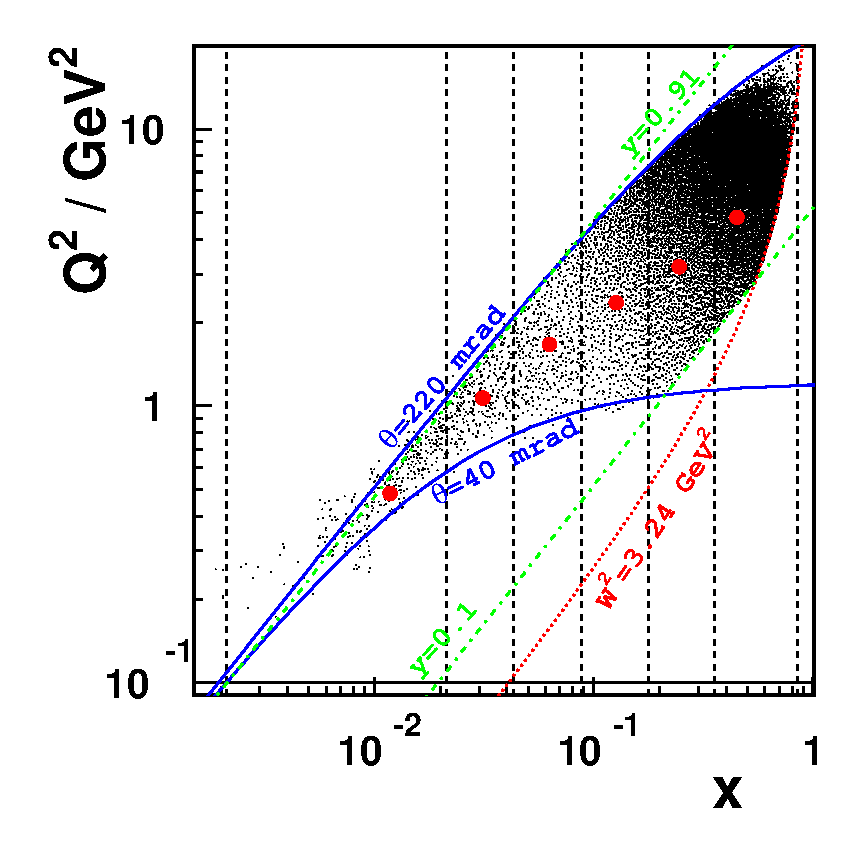
\includegraphics[angle=0,width=0.45\textwidth]{figs/kineplane.eps}
\caption{\label{HERMES_KIN} Kinematic coverage of the HERMES measurement.  The dashed vertical lines indicate the borders
of the bins in x, the dots their centers of gravity. The solid curves
indicate the
vertical acceptance of the spectrometer, defined by its aperture.
In addition, the
kinematic cuts imposed on the variables Q$^2$, y
and W$^2$ are shown. 
%The W$^2$ cut suppresses the nuclear resonance region.
{\it Reproduced from~\cite{Riedl:2005jq}.}}
\end{center}\end{figure}


The HERMES collaboration  made the first measurement~\cite{Riedl:2005jq,Airapetian:2005cb} of
$b_1$ in 2005.
The experiment explored the low $x$ region of $0.001<x<0.45$ for  $0.5<Q^2<5$ GeV$^2$.  
An atomic beam source was used to generate a deuterium gas target with high tensor polarization.  
The HERA storage ring provided 27.6 GeV positrons incident on the internal gas target.

As displayed in Fig.~\ref{HERMES_AZZ}, the tensor asymmetry A$_{zz}$  was found to be 
non-zero at about the  two sigma level, with an apparent zero crossing around $x=0.3$. %  for $x < 0.1$.  
%
The tensor structure function $b_1$ exhibits a steep rise as $x\to 0$, which is qualitatively
in agreement with the predictions of coherent double-scattering models. See for example Ref.~\cite{Edelmann:1997ik}.  The authors of Ref.~\cite{Airapetian:2005cb} interpret the rapid rise at low $x$ in terms of the same mechanism that leads to nuclear shadowing in unpolarized scattering, i.e. double scattering of the lepton, first from the proton, then from the neutron, with sensitivity to the spatial alignment of the two nucleons.
%The Close-Kumano integral (Eq.~\ref{cksum}) was evaluated and found to be:
%\begin{eqnarray}
%\int_{0.0002}^{0.85} b_1(x) dx = 0.0105 \pm 0.0034 \pm 0.0035
%\end{eqnarray}
%which result possibly indicates a breaking of the Close-Kumano sum rule, and consequently a 
%tensor-polarized quark sea.
%%
%%

As is often the case with a pioneer measurement, the precision of the results leaves some
room for ambiguity.  Despite the surprisingly large magnitude and interesting trend of the data, 
all points are roughly within two sigma from zero, which calls for a higher precision measurement.
Another issue is that some of the HERMES momentum transfer values are low 
(see Fig.~\ref{HERMES_KIN}), so that quark structure functions may not be the correct language. 
The $Q^2$ variation in each $x$-bin is also quite wide ($\approx$10 GeV$^2$ for $x\sim 0.3$), which complicates
the interpretation of this data, since  several models predict significant $Q^2$-dependence of
 $b_1$. See for example Fig.~\ref{xb1_pred}.



%\begin{figure}\begin{center}
%\includegraphics[angle=0,width=3.1in]{figs/b1g1.eps}
%\caption{\label{}\footnotesize
%{\it Reproduced from~\cite{Riedl:2005jq}.}}
%\end{center}\end{figure}

%\begin{figure}\begin{center}
%\includegraphics[angle=0,width=3.1in]{figs/b1g1overf1.eps}
%caption{\label{}\footnotesize
%{\it Reproduced from~\cite{Riedl:2005jq}.}}
%\end{center}\end{figure}

%\begin{figure}\begin{center}
%\includegraphics[angle=0,width=3.1in]{figs/b2theo.eps}
%\caption{\label{}\footnotesize
%{\it Reproduced from~\cite{Riedl:2005jq}.}}
%\end{center}\end{figure}


%%%%%%%%%%%%%
%%%%%%%%%%%%%
\subsubsection{Interpretation in the Operator Product Expansion}
%
In the Operator Product Expansion (OPE) framework, the leading operators 
$O_V^{\mu_1...\mu_n}$ and $O_A^{\mu_1...\mu_n}$ in the expansion are twist two. For a 
spin-1 target, the matrix elements of the time-ordered product of two currents 
$T_{\mu\nu}$ have the following expressions:
%
\begin{eqnarray}
<p,E|O_V^{\mu_1...\mu_n}|p,E>&=&S[a_np^{\mu_1}...p^{\mu_n}+d_n(E^{*\mu_1}E^{\mu_2}-\frac{1}{3}p^{\mu_1}
p^{\mu_2})p^{\mu_3}...p^{\mu_n}], \nonumber \\
<p,E|O_A^{\mu_1...\mu_n}|p,E>&=&S[r_n\epsilon^{\lambda\sigma\tau\mu_1}E_{\lambda}^*E_{\sigma}p_{\tau}
p^{\mu_2}...p^{\mu_n}]
\label{matrix-elt}
\end{eqnarray}
%
The non-zero value of $b_1$ arises from the fact that, in a spin-1 target, the 
$\frac{1}{3}p^{\mu_1}p^{\mu_2}$ term doesn't cancel the tensor structure $E^{*\mu_1}E^{\mu_2}$. 
The coefficient $d_n$ can be extracted from the comparison of $T_{\mu\nu}$ expansion 
and the spin-1 target hadronic tensor Eq.~\ref{had-tensor} as follows:
%
\begin{eqnarray}
b_1(\omega)&=&\sum_{n=2,4,...}^\infty 2 C_n^{(1)} d_n \omega^n, \nonumber \\
b_2(\omega)&=&\sum_{n=2,4,...}^\infty 4 C_n^{(2)} d_n \omega^{n-1},
\end{eqnarray}
%
for $1 \le |\omega| \le \infty$ (where $\omega = 1/x$). A Callan-Gross-type relation 
exists for the two leading order tensor structure functions:
%
\begin{eqnarray}
 2 x b_1 = b_2
\label{callan-gross}
\end{eqnarray}
%
valid at lowest order of QCD, where $C_n^{(1)} = C_n^{(2)}$.
At higher orders, Eq.~\ref{callan-gross} is violated.

Sum rules can be 
extracted from the moments of the tensor structure functions:
%
\begin{eqnarray}
\int_0^1 x^{n-1}~b_1(x)~dx &=& \frac{1}{2}~C_n^{(1)}~d_n, \nonumber \\
\int_0^1 x^{n-2}~b_2(x)~dx &=& C_n^{(2)}~d_n,
\label{sr}
\end{eqnarray}
%
where n is even. 

The OPE formalism is based on QCD and is target-independent. However, a target dependence 
is generated by Eq.~\ref{matrix-elt}, and spin-1 structure functions are subject to 
the same QCD corrections and their moments have the same anomalous dimensions as for 
a spin-1/2 target. In addition, the tensor structure functions should exhibit the same 
scaling behavior as $F_1$ and $F_2$, since they are generated from the same matrix 
element $O_V^{\mu_1...\mu_n}$.

We focus in this document on the leading twist structure function $b_1$.  A Callan-Gross type relation allows access to $b_2$ once $b_1$ is determined, and $b_3$ and $b_4$ do not contribute at leading twist.
%%%%%%%%
%%%%%%%%
\subsubsection{Interpretation in the Parton Model}
%
In the infinite momentum frame\footnote{All spins and
momenta are along the $z$-axis.} of the parton model, 
the scattering of the virtual photon from a free quark 
with spin up (or down), which carries a momentum fraction $x$ of the spin-$m$ hadron, can be 
expressed through the hadronic tensor $W_{\mu\nu}^{(m)}$:
%
\begin{eqnarray}
W_{\mu\nu}^{(1)} = \Bigg(- \frac{1}{2} g_{\mu\nu} + \frac{x}{\nu} P_{\mu}P{\nu}\Bigg) 
                               \Big(q^1_{\uparrow}(x) + q^1_{\downarrow}(x)\Big) \nonumber
                    + \frac{i \epsilon_{\mu\nu\lambda\sigma} q^{\lambda} s^{\sigma}}{2 \nu} 
                               \Big(q^1_{\uparrow}(x) - q^1_{\downarrow}(x)\Big),
\label{had-tensor-1}
\end{eqnarray}
%
for a target of spin projection equal to 1 along the $z$-direction, and:
%
\begin{eqnarray}
W_{\mu\nu}^{(0)} = \Bigg(- \frac{1}{2} g_{\mu\nu} + \frac{x}{\nu} P_{\mu}P{\nu}\Bigg) 
                               2 q^0_{\uparrow}(x) 
\label{had-tensor-0}
\end{eqnarray}
%
for a target of spin projection equal to zero along the $z$-direction. The tensor 
structure functions $b_1$ and $b_2$ can be expressed from the comparison of 
$W_{\mu\nu}^{(1)} - W_{\mu\nu}^{(0)}$ with Eq.~\ref{had-tensor} as follows:
%
\begin{eqnarray}
b_1(x) &=& \frac{1}{2} \Big( 2 q^0_{\uparrow}(x) - q^1_{\uparrow}(x) - q^1_{\downarrow}(x) \Big) \\
b_2(x) &=& 2 x b_1(x)
\label{TSF-parton}
\end{eqnarray}
%
where $q^m_{\uparrow}$ ($q^m_{\downarrow}$)  represents the probability to find a quark with momentum fraction $x$ and spin up (down) in a hadron which is in helicity state $m$.
%For example, $q^1_{\uparrow}(x)$ is the probability to find a quark with spin up and momentum fraction $x$ in a deuteron that is in state $m=1$. 
%
The tensor structure function $b_1$ depends only on the spin-averaged parton distributions\footnote{since, by parity, $q^m_{\uparrow}= q^m_{\downarrow}$} 
\begin{eqnarray*}
q^1(x) &=& q^1_{\uparrow}(x) + q^1_{\downarrow}(x)\\ 
q^0(x) &=& q^0_{\uparrow}(x) + q^0_{\downarrow}(x) 
= 2 q^0_{\uparrow}(x)
\end{eqnarray*}
so it can be expressed as:
\begin{eqnarray}
b_1(x) = \frac{q^0(x) - q^1(x)}{2}
\end{eqnarray}

Explicitly, $b_1$ measures the difference
in partonic constituency in an $|m|$=1 target and an $m$=0 target. 
 From this we see that while $b_1$ is defined in terms of quark distributions, it interestingly depends also on the spin state of the nucleus as a whole.

%The three leading twist structure functions are $F_1$, $g_1$ and $b_1$.
%The tensor structure function $b_1$, which is leading-twist like  $F_1$ and 
%$g_1$, is quite interesting, in that it presents a simple gauge of nuclear 
%effects: $b_1$ would vanish if the deuteron was simply a proton and neutron in 
%a relative S state.
%
%
%%The Hermes collaboration  made a first measurement~\cite{Airapetian:2005cb} of 
%$b_1$ and found significantly non-zero results.  Beyond providing insight into
%nuclear structure, this has the potential to impact $g_1^n$ and $g_2^n$ extractions, 
%where $b_1$ has traditionally been ignored when the neutron is extracted from 
%deuteron data.




